%!TEX TS-program = Arara
% arara: pdflatex: {shell: yes}
\documentclass[14pt,ngerman]{beamer}

\usepackage[T1]{fontenc}
\usepackage{booktabs}
\usepackage{babel}
\usepackage{graphicx}
\usepackage{csquotes}
\usepackage{xcolor}
\usepackage{tikz}
\usetikzlibrary{shapes}
\usetikzlibrary{shadows}
\usetikzlibrary{positioning}

\usepackage{listings}
\usepackage{bera}
 
\definecolor{colBack}{rgb}{1,1,0.8}
\definecolor{hellgelb}{rgb}{1,1,0.8}
\definecolor{colKeys}{rgb}{0,0,1}
\definecolor{colIdentifier}{rgb}{0,0,0}
\definecolor{colComments}{rgb}{1,0,0}
\definecolor{colString}{rgb}{0,0.5,0}
 
\lstset{%
    float=hbp,%
    basicstyle=\ttfamily\footnotesize, %
    identifierstyle=\color{colIdentifier}, %
    keywordstyle=\color{colKeys}, %
    stringstyle=\color{colString}, %
    commentstyle=\color{colComments}, %
    columns=flexible, %
    tabsize=2, %
    frame=single, %
    extendedchars=true, %
    showspaces=false, %
    showstringspaces=false, %
    numbers=left, %
    numberstyle=\tiny, %
    breaklines=true, %
    backgroundcolor=\color{colBack}, %
    breakautoindent=true, %
    captionpos=b,
    language={[LaTeX]TeX},
    morekeywords={draw,node,node,coordinate,grid,rounded,thick, corners,very,minimum,fill,width,height,rectangle,step,thin,readlist,foreachitem,setsepchar}
}
 

\lstset{literate=%
    {Ö}{{\"O}}1
    {Ä}{{\"A}}1
    {Ü}{{\"U}}1
    {ß}{{\ss}}1
    {ü}{{\"u}}1
    {ä}{{\"a}}1
    {ö}{{\"o}}1
    {~}{{\textasciitilde}}1
}

\author{Uwe Ziegenhagen}
\title{\textit{TikZ}ische Erlebnisse}
\subtitle{Dante Frühjahrstagung 2025}


\begin{document}

\begin{frame}

\maketitle

\end{frame}

\begin{frame}
\frametitle{Inhalt}

\begin{itemize}
\item Kurze (nicht vollständige) Vorstellung \newline von TikZ-Grundlagen
\item Beispiele, Beispiele, Beispiele\ldots 
\end{itemize}

\end{frame}

\section{Geschichte und Grundlagen} 

\begin{frame}
\frametitle{Geschichte}

\begin{itemize}
\item TikZ = \enquote{TikZ ist kein Zeichenprogramm}
\item TikZ = \enquote{Frontend} für PGF (\enquote{portable graphics format})
\item Entwickler Till Tantau, Christian Feuersänger
\item Erscheinungsjahr 2005
\end{itemize}
\end{frame}


\begin{frame}[containsverbatim]
\frametitle{Einfache Linien}

\begin{lstlisting}
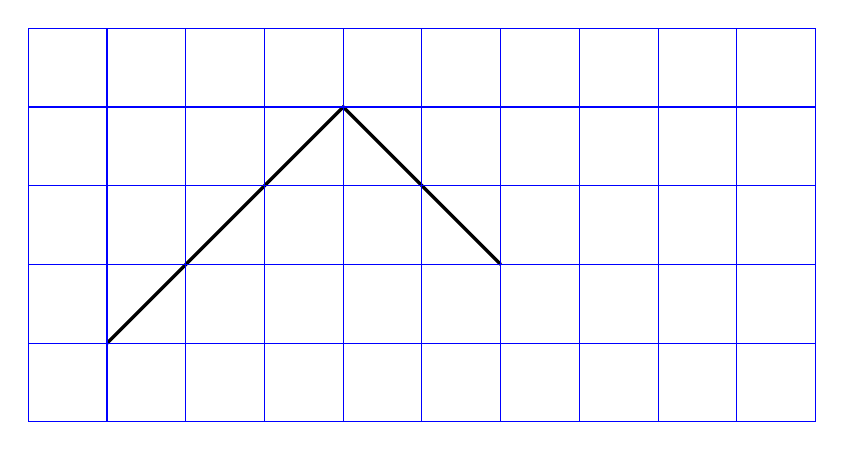
\begin{tikzpicture}
\draw[very thick] (1,1) -- (4,4) -- (6,2);
\draw[step=1cm,blue,thin] (0,0) grid (10,5);
\end{tikzpicture}
\end{lstlisting}

\begin{center}
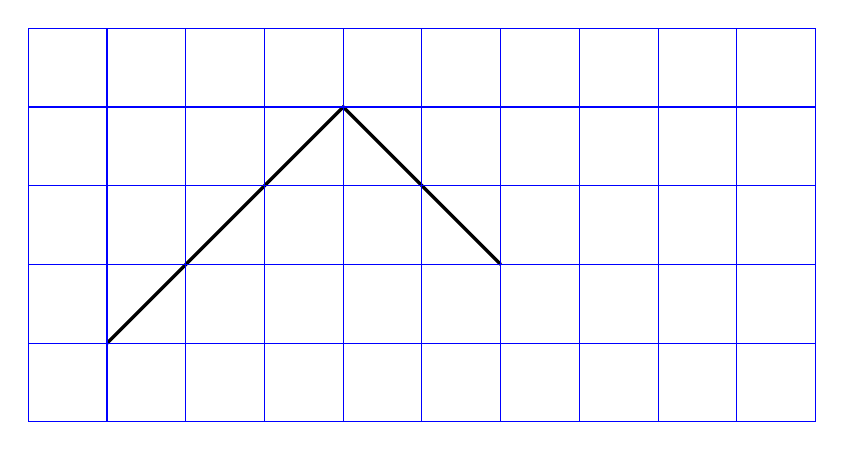
\begin{tikzpicture}
\draw[very thick] (1,1) -- (4,4) -- (6,2);
\draw[step=1cm,blue,thin] (0,0) grid (10,5);
\end{tikzpicture}
\end{center}


\end{frame}


\begin{frame}[containsverbatim]
\frametitle{Liniendicken}

\begin{lstlisting}

\begin{tikzpicture}
\draw[ultra thin] (2,1) -- (2,3);
\draw[very thin] (2.5,1) -- (2.5,3);
\draw[thin] (3,1) -- (3,3);
\draw[semithick] (3.5,1) -- (3.5,3);
\draw[thick] (4,1) -- (4,3);
\draw[very thick] (4.5,1) -- (4.5,3);
\draw[ultra thick] (5,1) -- (5,3);
\draw[line width=4pt] (5.5,1) -- (5.5,3);
\end{tikzpicture}
\end{lstlisting}

\begin{center}

\begin{tikzpicture}
\draw[ultra thin] (2,1) -- (2,3);
\draw[very thin] (2.5,1) -- (2.5,3);
\draw[thin] (3,1) -- (3,3);
\draw[semithick] (3.5,1) -- (3.5,3);
\draw[thick] (4,1) -- (4,3);
\draw[very thick] (4.5,1) -- (4.5,3);
\draw[ultra thick] (5,1) -- (5,3);
\draw[line width=4pt] (5.5,1) -- (5.5,3);
\end{tikzpicture}
\end{center}


\end{frame}

\begin{frame}[containsverbatim]
\frametitle{Linienstile}

\begin{lstlisting}
\begin{tikzpicture}
\draw[thick, dashed] (2,1) -- (2,3);
\draw[thick, loosely dashed] (2.5,1) -- (2.5,3);
\draw[thick, densely dashed] (3,1) -- (3,3);
\draw[thick, dotted] (3.5,1) -- (3.5,3);
\draw[thick, loosely dotted] (4,1) -- (4,3);
\draw[thick, densely dotted] (4.5,1) -- (4.5,3);
\end{tikzpicture}
\end{lstlisting}


\begin{center}
\begin{tikzpicture}
\draw[thick, dashed] (2,1) -- (2,3);
\draw[thick, loosely dashed] (2.5,1) -- (2.5,3);
\draw[thick, densely dashed] (3,1) -- (3,3);
\draw[thick, dotted] (3.5,1) -- (3.5,3);
\draw[thick, loosely dotted] (4,1) -- (4,3);
\draw[thick, densely dotted] (4.5,1) -- (4.5,3);
\end{tikzpicture}
\end{center}


\end{frame}



\begin{frame}[containsverbatim]
\frametitle{Rel. Koordinaten I}

mit Update der Koordinaten

\begin{lstlisting}[basicstyle=\ttfamily\scriptsize]
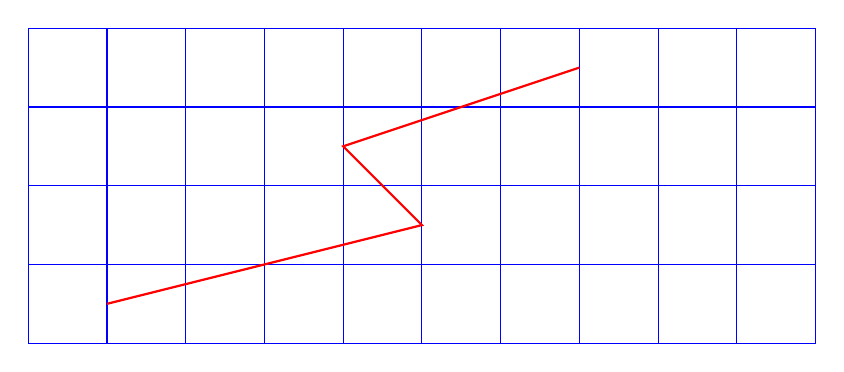
\begin{tikzpicture}
\draw[step=1cm,blue,thin] (0,0) grid (10,4);

\draw[thick, red] (1,0.5) -- ++(4,1) -- ++(-1,1) -- ++(3,1);
\end{tikzpicture}
\end{lstlisting}

\begin{center}
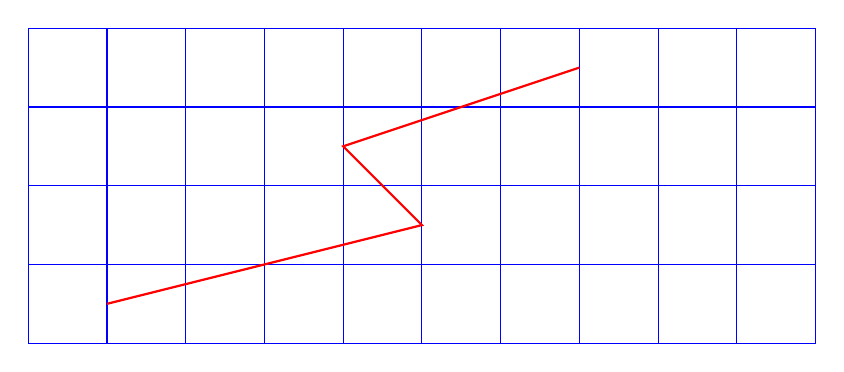
\begin{tikzpicture}
\draw[step=1cm,blue,thin] (0,0) grid (10,4);

\draw[thick, red] (1,0.5) -- ++(4,1) -- ++(-1,1) -- ++(3,1);
\end{tikzpicture}
\end{center}

\end{frame}


\begin{frame}[containsverbatim]
\frametitle{Rel. Koordinaten II}

ohne Update der Koordinaten

\begin{lstlisting}[basicstyle=\ttfamily\scriptsize]
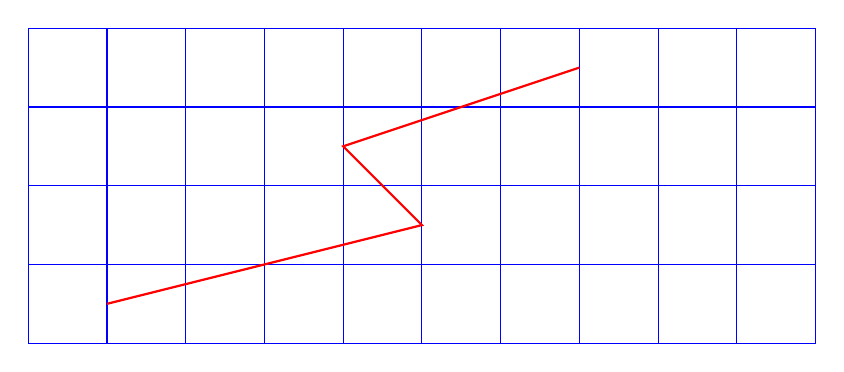
\begin{tikzpicture}
\draw[step=1cm,blue,thin] (0,0) grid (10,4);

\draw[thick, red] (1,0.5) -- ++(4,1) -- ++(-1,1) -- ++(3,1);
\end{tikzpicture}
\end{lstlisting}


\begin{center}
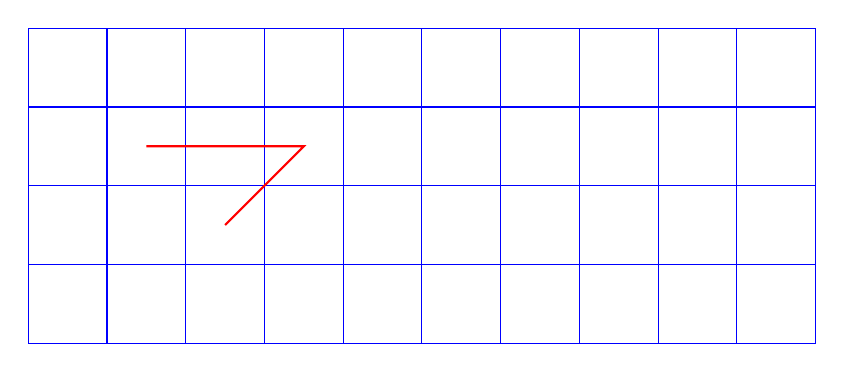
\begin{tikzpicture}
\draw[step=1cm,blue,thin] (0,0) grid (10,4);

%\draw[thick, red] (2.5,2.5) -- ++(1,1) -- ++(-1,1);

\draw[thick, red] (2.5,1.5) -- +(1,1) -- +(-1,1);
\end{tikzpicture}
\end{center}

\end{frame}


\begin{frame}[containsverbatim]
\frametitle{Nodes und Coordinates}

\begin{lstlisting}[basicstyle=\ttfamily\scriptsize]
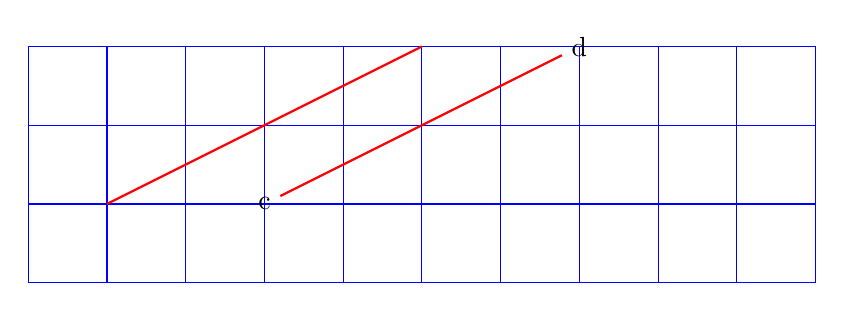
\begin{tikzpicture}
\draw[step=1cm,blue,thin] (0,0) grid (10,3);

\coordinate (a) at (1,1);
\coordinate (b) at (5,3);
\draw[red, thick] (a) -- (b);

\node (c) at (3,1){c};
\node (d) at (7,3){d};
\draw[red, thick] (c) -- (d);
\end{tikzpicture}
\end{lstlisting}

\begin{center}
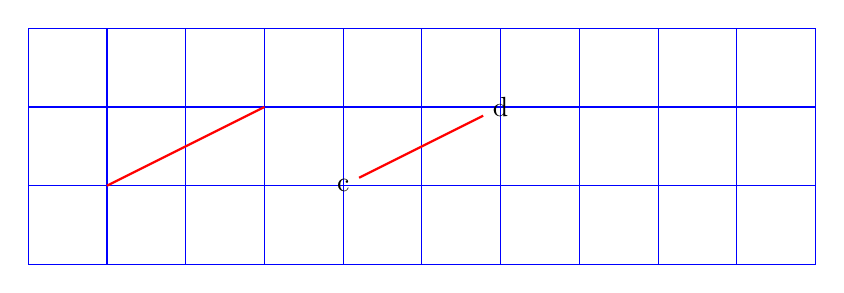
\begin{tikzpicture}
\draw[step=1cm,blue,thin] (0,0) grid (10,3);

\coordinate (a) at (1,1);
\coordinate (b) at (3,2);
\draw[red, thick] (a) -- (b);

\node (c) at (4,1){c};
\node (d) at (6,2){d};
\draw[red, thick] (c) -- (d);
\end{tikzpicture}
\end{center}

\end{frame}




\begin{frame}[containsverbatim]
\frametitle{Node Shapes}

\begin{lstlisting}[basicstyle=\ttfamily\scriptsize]
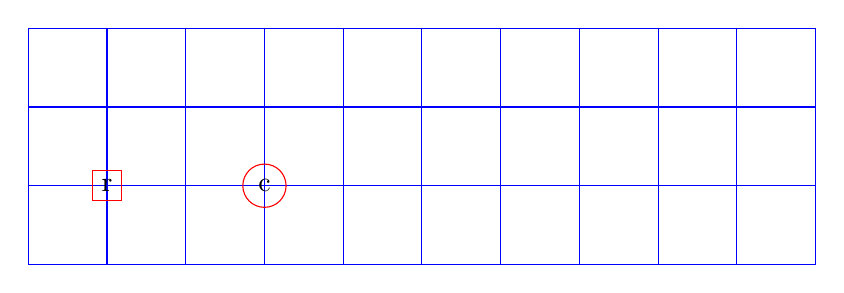
\begin{tikzpicture}
\draw[step=1cm,blue,thin] (0,0) grid (10,3);

\node[rectangle,draw = red] (r) at (1,1){r};
\node[circle,draw = red] (c) at (3,1){c};
\end{tikzpicture}
\end{lstlisting}

\begin{center}
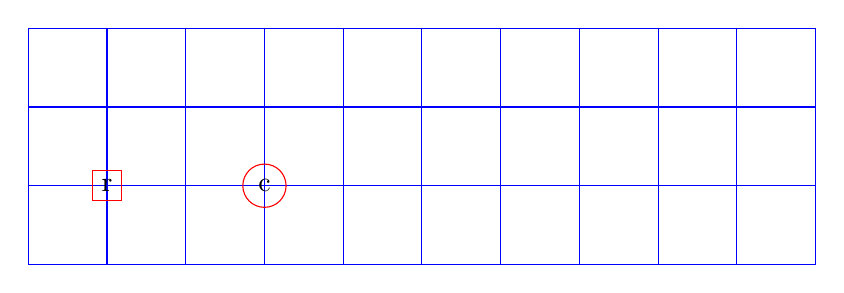
\begin{tikzpicture}
\draw[step=1cm,blue,thin] (0,0) grid (10,3);

\node[rectangle,draw = red] (r) at (1,1){r};
\node[circle,draw = red] (c) at (3,1){c};
\end{tikzpicture}
\end{center}

\begin{itemize}
	\item more with \verb|\usetikzlibrary{shapes}|
\end{itemize}

\end{frame}




\begin{frame}[containsverbatim]
\frametitle{Mehr Node Shapes}

\begin{lstlisting}[basicstyle=\ttfamily\scriptsize]
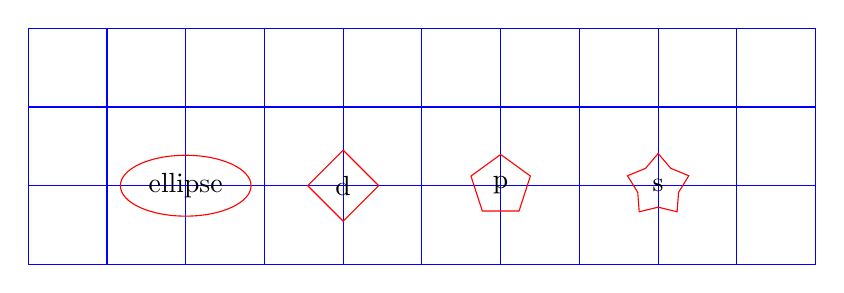
\begin{tikzpicture}
\draw[step=1cm,blue,thin] (0,0) grid (10,3);

\node[ellipse,draw = red] (e) at (2,1){ellipse};
\node[diamond,draw = red] (d) at (4,1){d};
\node[regular polygon,regular polygon sides=5,draw=red](p) at (6,1){p};
\node[star,star points=5,draw = red] (s) at (8,1){s};
\end{tikzpicture}
\end{lstlisting}

\begin{center}
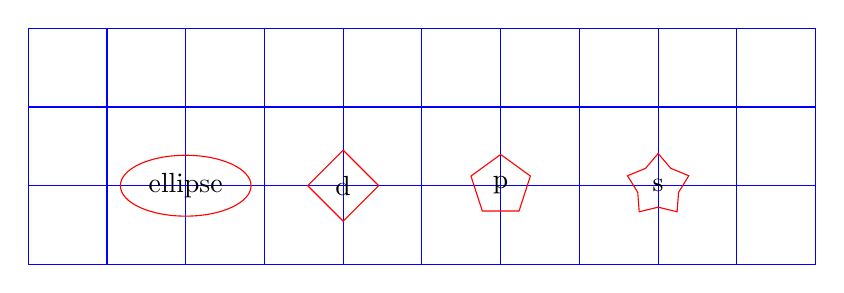
\begin{tikzpicture}
\draw[step=1cm,blue,thin] (0,0) grid (10,3);

\node[ellipse,draw = red] (e) at (2,1){ellipse};
\node[diamond,draw = red] (d) at (4,1){d};
\node[regular polygon,regular polygon sides=5,draw=red](p) at (6,1){p};
\node[star,star points=5,draw = red] (s) at (8,1){s};
\end{tikzpicture}
\end{center}

\end{frame}

\begin{frame}[containsverbatim]
\frametitle{Shapes formatieren}

\begin{lstlisting}[basicstyle=\ttfamily\scriptsize]
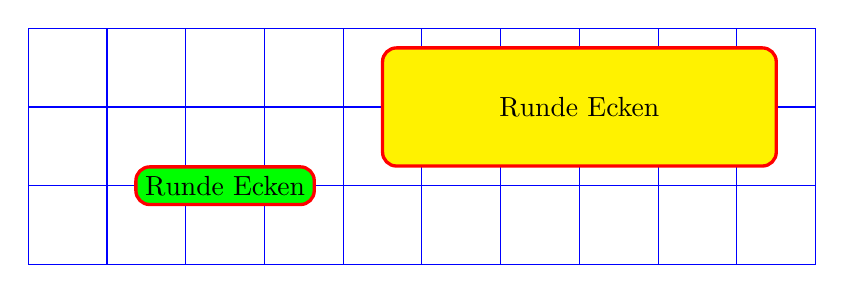
\begin{tikzpicture}
\draw[step=1cm,blue,thin] (0,0) grid (10,3);

\node[rectangle,draw = red,very thick,rounded corners=5pt,fill=green] (r) at (2.5,1){Runde Ecken};

\node[rectangle,draw = red,very thick,rounded corners=5pt,minimum width=5cm, minimum height=15mm, fill=yellow] (r) at (7,2){Runde Ecken};
\end{tikzpicture}
\end{lstlisting}

\begin{center}
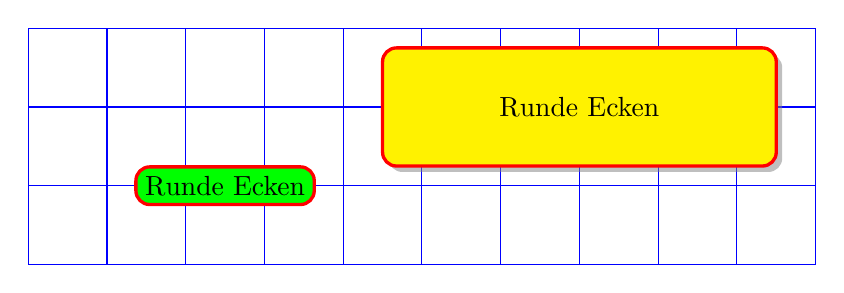
\begin{tikzpicture}
\draw[step=1cm,blue,thin] (0,0) grid (10,3);

\node[rectangle,draw = red,very thick,rounded corners=5pt,fill=green] (r) at (2.5,1){Runde Ecken};

\node[rectangle,drop shadow,draw = red,very thick,rounded corners=5pt,minimum width=5cm, minimum height=15mm, fill=yellow] (r) at (7,2){Runde Ecken};
\end{tikzpicture}
\end{center}

\end{frame}


\begin{frame}
\frametitle{Grundlagen II}

Anchors
\end{frame}

\begin{frame}
\frametitle{Anwendungen}

\begin{itemize}
	\item Zielscheibe 10m Luftpistole
	\item Matrix
	\item Kalender
	\item 
	\item 
	\item 
	\end{itemize}

\end{frame}


\begin{frame}[containsverbatim]
\frametitle{Zielscheibe Luftpistole I} % [basicstyle=\ttfamily\scriptsize]

\begin{lstlisting}
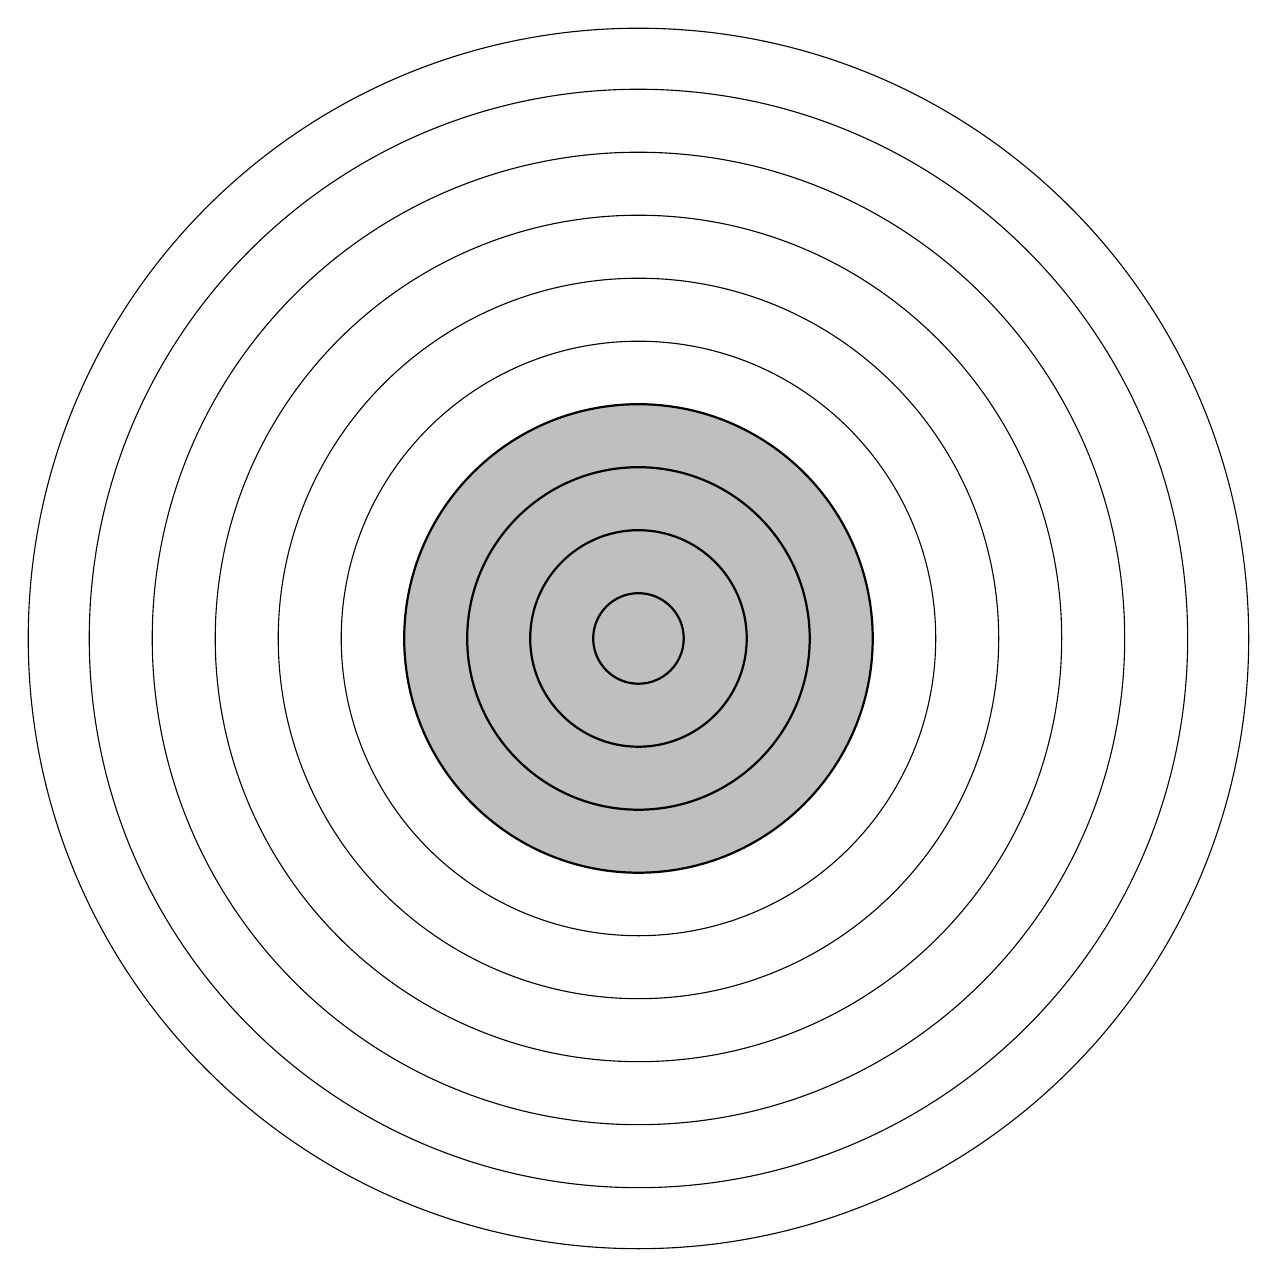
\begin{tikzpicture}
\coordinate (o) at (8,8);
\draw[black] (o) circle (77.5mm);
\draw[black] (o) circle (69.75mm);
\draw[black] (o) circle (61.75mm);
\draw[black] (o) circle (53.75mm);
\draw[black] (o) circle (45.75mm);
\draw[black] (o) circle (37.75mm);
\draw[black,thick,fill=lightgray] (o) circle (29.75mm);
\draw[black,thick] (o) circle (21.75mm);
\draw[black,thick] (o) circle (13.75mm);
\draw[black,thick] (o) circle (5.75mm);
\end{tikzpicture}
\end{lstlisting}

\end{frame}



\begin{frame}[containsverbatim]
\frametitle{Zielscheibe Luftpistole II}

\begin{center}
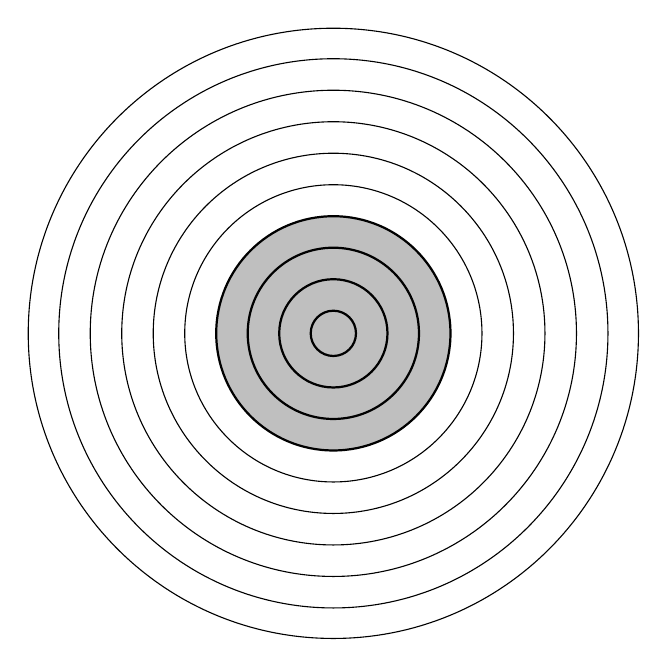
\begin{tikzpicture}[scale=0.5]
\coordinate (o) at (8,8);
\draw[black] (o) circle (77.5mm);
\draw[black] (o) circle (69.75mm);
\draw[black] (o) circle (61.75mm);
\draw[black] (o) circle (53.75mm);
\draw[black] (o) circle (45.75mm);
\draw[black] (o) circle (37.75mm);
\draw[black,thick,fill=lightgray] (o) circle (29.75mm);
\draw[black,thick] (o) circle (21.75mm);
\draw[black,thick] (o) circle (13.75mm);
\draw[black,thick] (o) circle (5.75mm);
\end{tikzpicture}
\end{center}

\end{frame}


\begin{frame}[containsverbatim]
\frametitle{Zielscheibe Luftpistole III} % [basicstyle=\ttfamily\scriptsize]

\begin{itemize}
	\item Positioning-Bibliothek laden
\end{itemize}


\begin{lstlisting}
\usetikzlibrary{positioning} 
\end{lstlisting}

\begin{lstlisting}
\begin{tikzpicture}
\node[right=0.7cm of o] {9};
\node[right=1.5cm of o] {8};
\node[right=2.3cm of o] {7};
\node[right=3.1cm of o] {6};
\node[right=3.9cm of o] {5};
\node[right=4.7cm of o] {4};
\node[right=5.5cm of o] {3};
\node[right=6.3cm of o] {2};
\node[right=7.1cm of o] {1};
\end{tikzpicture}
\end{lstlisting}\vspace*{-0.2cm}

\begin{itemize}
	\item wiederholen für left, above, below
\end{itemize}
\end{frame}

\begin{frame}[containsverbatim]
\frametitle{Zielscheibe Luftpistole IV}

\begin{center}
\resizebox{8cm}{8cm}{%
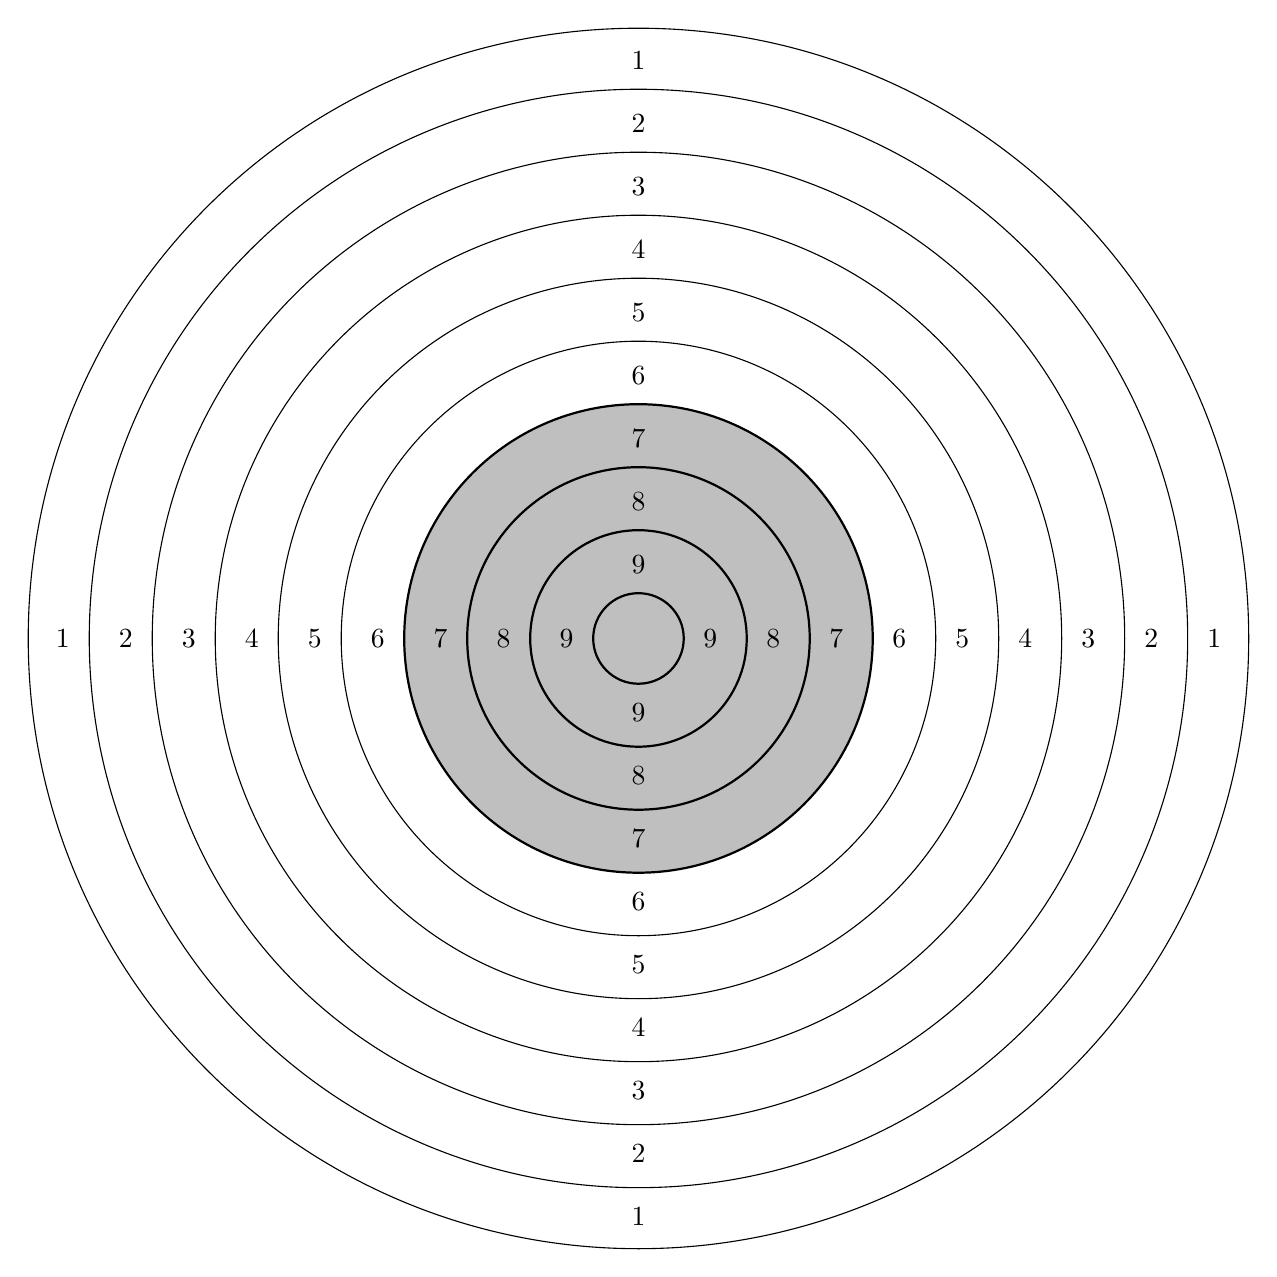
\begin{tikzpicture}
\coordinate (o) at (8,8);
\draw[black] (o) circle (77.5mm);
\draw[black] (o) circle (69.75mm);
\draw[black] (o) circle (61.75mm);
\draw[black] (o) circle (53.75mm);
\draw[black] (o) circle (45.75mm);
\draw[black] (o) circle (37.75mm);
\draw[black,thick,fill=lightgray] (o) circle (29.75mm);
\draw[black,thick] (o) circle (21.75mm);
\draw[black,thick] (o) circle (13.75mm);
\draw[black,thick] (o) circle (5.75mm);

\node[right=0.7cm of o] {9};
\node[right=1.5cm of o] {8};
\node[right=2.3cm of o] {7};
\node[right=3.1cm of o] {6};
\node[right=3.9cm of o] {5};
\node[right=4.7cm of o] {4};
\node[right=5.5cm of o] {3};
\node[right=6.3cm of o] {2};
\node[right=7.1cm of o] {1};

\node[above=0.7cm of o] {9};
\node[above=1.5cm of o] {8};
\node[above=2.3cm of o] {7};
\node[above=3.1cm of o] {6};
\node[above=3.9cm of o] {5};
\node[above=4.7cm of o] {4};
\node[above=5.5cm of o] {3};
\node[above=6.3cm of o] {2};
\node[above=7.1cm of o] {1};

\node[left=0.7cm of o] {9};
\node[left=1.5cm of o] {8};
\node[left=2.3cm of o] {7};
\node[left=3.1cm of o] {6};
\node[left=3.9cm of o] {5};
\node[left=4.7cm of o] {4};
\node[left=5.5cm of o] {3};
\node[left=6.3cm of o] {2};
\node[left=7.1cm of o] {1};


\node[below=0.7cm of o] {9};
\node[below=1.5cm of o] {8};
\node[below=2.3cm of o] {7};
\node[below=3.1cm of o] {6};
\node[below=3.9cm of o] {5};
\node[below=4.7cm of o] {4};
\node[below=5.5cm of o] {3};
\node[below=6.3cm of o] {2};
\node[below=7.1cm of o] {1};
\end{tikzpicture}}
\end{center}

\end{frame}

\begin{frame}[containsverbatim]
\frametitle{Zielscheibe Luftpistole V}

\begin{itemize}
\item Code vereinfachen mit \texttt{listofitems} Paket
\end{itemize}


\begin{lstlisting}
\usepackage{listofitems}
\setsepchar{;}
\coordinate (o) at (8,8);
\draw[black,thick,fill=lightgray] (o) circle (29.75mm);
\readlist\distances{77.5;69.75;61.75;53.75;45.75;37.75;21.75;13.75;5.75}
\foreachitem\distance\in\distances{
	\draw[black] (o) circle (\distance mm);
}
\readlist\distances{7.1;6.3;5.5;4.7;3.9;3.1;2.3;1.5;0.7}
\readlist\directions{right;above;left;below}
\foreachitem\direction\in\directions{
  \foreachitem\distance\in\distances{
    \node[\direction=\distance cm of o] {\distancecnt};
   }}
\end{lstlisting}


\end{frame}




\end{document}